\documentclass{article}
\usepackage[LGR, T1]{fontenc}
\usepackage[greek]{babel}
\usepackage{cancel}
\usepackage{amsmath}
\usepackage{tikz}
\usetikzlibrary{trees}
\usetikzlibrary{shapes.geometric,arrows}
\usetikzlibrary{calc}
\tikzset{
    treenode/.style={align=center, inner sep=1pt, text centered},
    root/.style={treenode, fill=blue!20, isosceles triangle, draw=blue,rotate=90, isosceles triangle apex angle=60, minimum height=0.7cm, minimum width=0.8cm},
    chance/.style={treenode, fill=red!20, circle, draw=red, minimum size=0.6cm},
    min/.style={treenode, fill=red, isosceles triangle,rotate=270, isosceles triangle apex angle=60, minimum height=0.7cm, minimum width=0.8cm},
    leaf/.style={treenode, minimum size=0.3cm}
}
\begin{document}
\title{\textlatin{question3}}
\maketitle


\section*{ΑΠΑΝΤΗΣΗ:}
\subsection*{(α):}
Θα αντιγράψουμε το δέντρο και θα υπολογίσουμε τις τιμές των εσωτερικών κόμβων. Οι \textlatin{MIN} κόμβοι θα πάρουν την ελάχιστη τιμή από τα φύλλα και οι κόμβοι τύχης τις αναμενόμενες τιμές \textlatin{minimax}. Τέλος, φαίνεται με ένα βελάκι ποια είναι η καλύτερη κίνηση για την ρίζα.

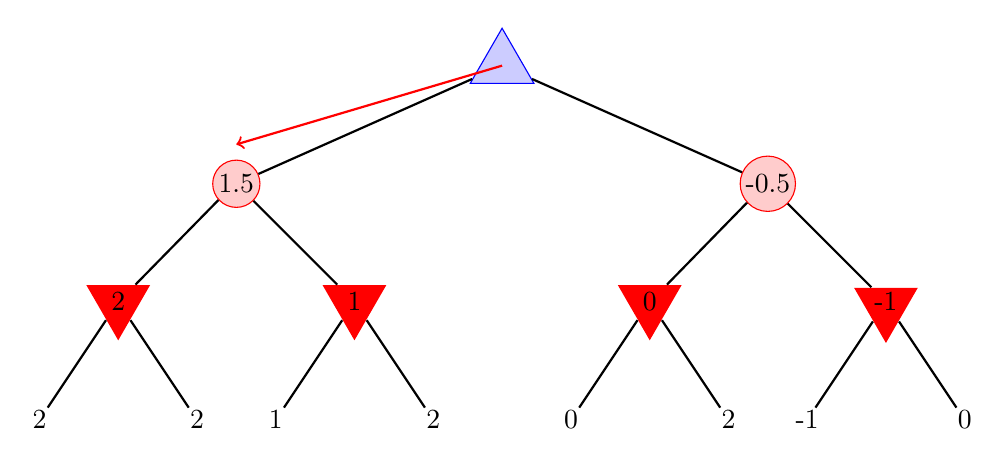
\begin{tikzpicture}[
  level 1/.style={sibling distance=6.75cm,},
  level 2/.style={sibling distance=3cm,},
  level 3/.style={sibling distance=2cm,},
  level 4/.style={sibling distance=0.4cm,}, 
  sibling distance=5cm,
  every node/.style={treenode}, 
  edge from parent/.style={draw, thick}]

\node[root] (root) {}
    child {node[chance] (c1) {1.5}
        child {node[min] {\rotatebox{90}{2}}
            child {node[leaf] {2}}
            child {node[leaf] {2}}
        }
        child {node[min] {\rotatebox{90}{1}}
            child {node[leaf] {1}}
            child {node[leaf] {2}}
        }
    }
    child {node[chance] {-0.5}
        child {node[min] {\rotatebox{90}{0}}
            child {node[leaf] {0}}
            child {node[leaf] {2}}
        }
        child {node[min] {\rotatebox{90}{-1}}
            child {node[leaf] {-1}}
            child {node[leaf] {0}}
        }
    };
    \draw[->, red, thick, bend left=0] ($(root)$) to[bend left] ($(c1)+(0,0.5)$);

\end{tikzpicture}
\subsection*{(β):}
Αν μας δώσουν τα πρώτα 6 φύλλα,  χρειάζεται να υπολογίσουμε τις τιμές του έβδομου και του όγδοου κατά την εύρεση της καλύτερης κίνησης για τη ρίζα. 
\\ \\
Αυτό διότι αν πχ η τιμή και των δύο φύλλων (7ο και 8ο)
ήταν \(+\infty\), τότε και το \textlatin{min node} θα έπαιρνε \textlatin{value} \(+\infty\), όμοια και το \textlatin{chance node}, άρα στην ρίζα θα ήταν καλύτερη επιλογή ο δεξιός κόμβος \textlatin{max}(1.5, \(+\infty\))
\\ \\ 
Ας υποθέσουμε τώρα ότι μας δίνουν τα πρώτα 7 φύλλα.
\\
Ο αριστερός κόμβος τύχης δεν αλλάζει, θα έχει τιμή 1,5.
\\
Για τον δεξιό κόμβο τύχης, το αριστερό \textlatin{min node} θα έχει τιμή 0 ( \textlatin{min}(0, 2) ).
\\
Για τον δεύτερο \textlatin{min node}, έχουμε -1 ως πρώτο φύλλο.
\\ \\
Έχει σημασία το 8ο φύλλο? Όχι, διότι ακόμη και αν είναι \(+\infty\), ο \textlatin{min} θα επιλέξει το -1 και ρίζα θα επιλέξει \textlatin{max}(1.5, -0.5) = 1.5 όπως πριν.
Αν πάλι το 8ο φύλλο ήταν \(-\infty\), τοτε ο δεξής κόμβος τύχης θα είχε \textlatin{value} \(-\infty\) και η ρίζα θα επιλέξει \textlatin{max}(1.5, \(-\infty\)) = 1.5 όπως πριν.
Άρα ανεξάρτητα από το 8ο φύλλο το αποτέλεσμα είναι προκαθορισμένο. 

\subsection*{(γ):}
Μετά τα δύο πρώτα φύλλα (και τα δύο 2), πιθανές τιμές για τον αριστερό κόμβο τύχης:\\ 
Ο αριστερός κόμβος \textlatin{min} έχει τιμή 2 (\textlatin{min} από {2,2}). \\
Ο δεξιός κόμβος \textlatin{min} θα μπορούσε να πάρει οποιαδήποτε τιμή στο [-2,2] (καθώς αυτές είναι οι πιθανές τιμές των φύλλων, προφανώς και ο μέσος όρος τους παίρνει οποιαδήποτε τιμή από αυτές). \\
Ο κόμβος τύχης παίρνει το μέσο όρο του 2 και της τιμής του δεξή κόμβου \textlatin{min}.
Χειρότερη περίπτωση (και τα 2 φύλλα παίρνουν την ελάχιστη τιμή -2) : Ο αριστερός κόμβος τύχης έχει ελάχιστη τιμή \((2 + -2)/2 = 0\) \\
Καλύτερη περίπτωση (και τα 2 φύλλα παίρνουν την μέγιστη τιμή 2) : Ο αριστερός κόμβος τύχης έχει μέγιστη τιμή \((2 + 2)/2 = 2\) \\
\\
Επομένως, ο αριστερός κόμβος τύχης παίρνει οποιαδήποτε τιμή στο [0, 2]. \\
\subsection*{(δ)}
Δεδομένου του περιορισμού [-2,2] και ενός αλγορίθμου τύπου κλαδέματος άλφα-β:\\
\\
Είναι εύκολο να δει κανείς ότι θα χρειαστεί να υπολογίσουμε όλο το αριστερό υπόδεντρο, δεν γίνεται κάποιο κλάδεμα εκεί.
\\
Όμως στο δεξί υπόδεντρο:
Ο πρώτος κόμβος \textlatin{min} δίνει το πολύ 0 \\
Ο δεξιός κόμβος \textlatin{min} μπορεί στην καλύτερη περίπτωση να δώσει 2 \\
Άρα ο μέσος όρος που θα δώσει την \textlatin{expectimax} τιμή στον δεξιό κόμβο τύχης παίρνει μέγιστη τιμή 1 (0 και οτιδήποτε \(\leq\) 2) \\
Επομένως, ο δεξιός κόμβος τύχης δεν μπορεί με τίποτα να "νικήσει" το 1,5 \\
\\
Επομένως, μπορούμε να κλαδέψουμε το δεξιό κόμβο \textlatin{min} και τα παιδιά του, καθώς και το άλλο φύλλο του αριστερού κόμβου \textlatin{min}. Παρακάτω φαίνονται κυκλωμένοι οι κλαδευμένοι κόμβοι.\\
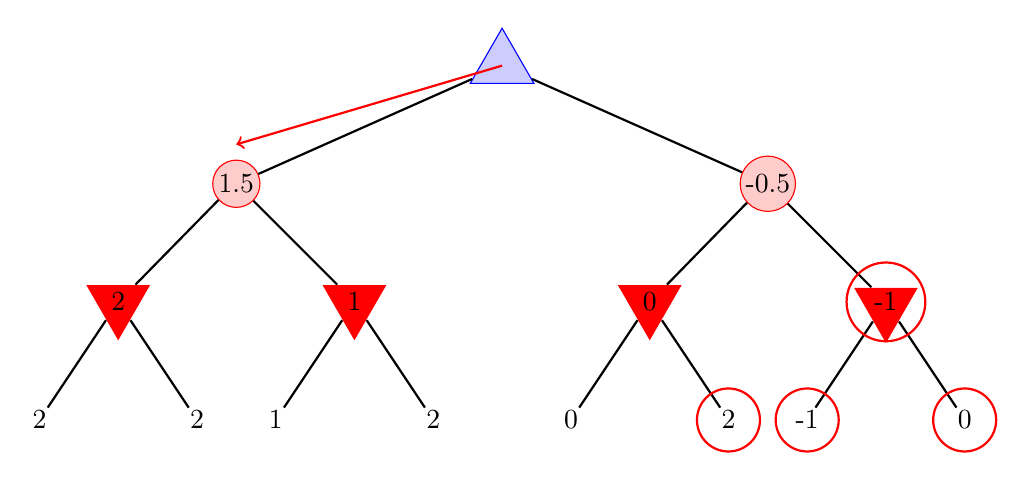
\begin{tikzpicture}[
  level 1/.style={sibling distance=6.75cm,},
  level 2/.style={sibling distance=3cm,},
  level 3/.style={sibling distance=2cm,},
  level 4/.style={sibling distance=0.4cm,}, 
  sibling distance=5cm, % Wider sibling distance
  every node/.style={treenode}, 
  edge from parent/.style={draw, thick}]

\node[root] (root) {}
    child {node[chance] (c1) {1.5}
        child {node[min] {\rotatebox{90}{2}}
            child {node[leaf] {2}}
            child {node[leaf] {2}}
        }
        child {node[min] {\rotatebox{90}{1}}
            child {node[leaf] {1}}
            child {node[leaf] {2}}
        }
    }
    child {node[chance] {-0.5}
        child {node[min] {\rotatebox{90}{0}}
            child {node[leaf] {0}}
            child {node[leaf] (p4) {2}}
        }
        child {node[min] (p1) {\rotatebox{90}{-1}}
            child {node[leaf] (p2) {-1}}
            child {node[leaf] (p3) {0}}
        }
    };

\draw[circle, red, thick] (p1) circle (0.5cm);
\draw[circle, red, thick] (p2) circle (0.4cm);
\draw[circle, red, thick] (p3) circle (0.4cm);
\draw[circle, red, thick] (p4) circle (0.4cm);

\draw[->, red, thick, bend left=0] ($(root)$) to[bend left] ($(c1)+(0,0.5)$);

\end{tikzpicture}
\end{document}
